%  <-- ezzel lesznek jelölve a kommentek,
%a legtöbb dolgot jobb békénhagyni úgy ahogy van, általában csak {} közé vagy \section{} alá kell írni majd
%az ITKproc miatt nem kell megformáznod a szöveget tehát ezt mindenképpen hagyjátok a itt, valamint mindig legyen a dokumentum mappájában, hogy elérje a fordító
\documentclass[10pt, conference, a4paper]{ITKproc}

\usepackage[utf8]{inputenc}
\usepackage{graphicx}
\usepackage{gensymb}
\graphicspath{ {images/} }
% correct bad hyphenation here

\hyphenation{pre-sence vi-su-alized si-mu-la-tions mo-le-cu-lar se-ve-ral cha-rac-te-ris-tic CoNSEnsX}


\begin{document}
% ide a {} közé írd a jegyzőkönyv címét
\title{Mikrokontroller II. mérési jegyzőkönyv}
% ezek gondolom egyértelműek, itt is mindig csak a {} szerkesszétek, valamint használhattok \\ sortöréshez, pl dátum hozzáírás stb
\author{\IEEEauthorblockN{Mátyás ANTAL}
\IEEEauthorblockA{(Supervisor: Attila TIHANYI)\\
Pázmány Péter Catholic University, Faculty of Information Technology and Bionics\\
50/a Pr\'ater street, 1083 Budapest, Hungary\\
\texttt{antal.matyas.gergely@hallgato.ppke.hu}}
}


\maketitle

\begin{abstract}
A mérés célja volt a mikrokontrollerek gyakorlati megismerése, az MSP 430-196 mikrokontroller használata, egyszerű alapműveletek végrehajtása, ezzel a flag bitek működésének gyakorlati vizsgálata. 
\end{abstract}

\IEEEpeerreviewmaketitle
% innentől kezdve jönnek a feladatok
% \section{} Ezzel hozunk létre fejezetet, a {} közé pedig bármi írhatunk, általában úgyis "Feladat" és "összefoglalás"-t fogunk,
% a fejezetek alapjáraton számozódnak római számokkal tehát azt nem szükséges beleírni, 
% ha alfejezeteket akarunk létrehozni akkor \subsection{} subsubsection{} stb- vel tegyük
%példa:
\section{Mérendő objektumok}

A mérés során az MSP 430-196 mikrokontrollert, valamint egy számítógépet és az ezen futó programozási környezetet használtunk, ennek segítségével végeztünk a mikrokontrolleren egyszerű alapműveleteket, összeadást és kivonást, ezzel ismerkedve a műveletvégzéssel, valamint a flagek használatával. A mérés során a műveletek elvégzésére használt programrészleteket a jegyzőkönyvbe illesztem, valamint az elkészült programot az emailhez csatolom. 

\section{LED kigyújtása}
Az első feladat megvalósítására a mérési utasításban kapott példaprogram alkalmas volt, így ennek működését vizsgáltuk. A kódrészlet első két parancsa nullázza a P2Out és a P2DIR 1-es bitjét, ezzel kikapcsolva a LED-et. A bit.b parancs a carry bitbe tölti a joystick P2IN gombjának helyzetét. Gombnyomás esetén ennek értéke 0, különben 1. A jc paranccsal visszaugrunk a program elejére, ha a carry 1, vagyis nem történt gombnyomás. A parancs miatt a program csak akkor jut tovább, ha az előző feltétel hamis volt, azaz a gombot megnyomtuk, ekkor a LED kigyullad. Ezután a program visszaugrik az elejére, várva a következő gombnyomást. 

\begin{figure}[h]
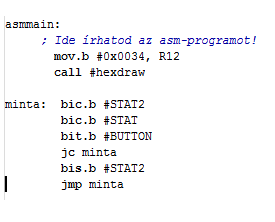
\includegraphics[scale=0.65]{legelso}
\centering
\end{figure}

\section{Szám növelése gombnyomásra}

A feladat megoldásához az R4 regiszterbe töltöttük a kezdőértéket, ezt fogjuk később növelni. A feladatban az értéket az R12 regiszterbe töltöttük, majd a $hexdraw$ függvény segítségével a képernyőre írattuk. Az előző feladathoz hasonlóan minden ciklusonban ellenőriztük a nyomógomb értékét a carry flagbe töltve. Amennyiben nem történt gombnyomás, a jc paranccsal a program elejére ugrottunk. Amennyiben a gombot megnyomtuk, az inc.b parancs segítségével az R4 értékét eggyel megnöveltük, majd az R12 regiszterbe töltve, a $hexdraw$ függvény ismételt használatával kirajzoltattuk. \\
Mivel egy gombnyomás ideje alatt több ciklus is lefuthatott, nehéz volt a számot egyesével növelni. Ennek megoldására hoztuk létre a $nyomom$ függvényt, mely a gomb elengedéséig nem engedte a program újraindulását. Ezzel értük el, hogy egy gombnyomás csak egy számnövelést eredményezzen. 

\begin{figure}[h]
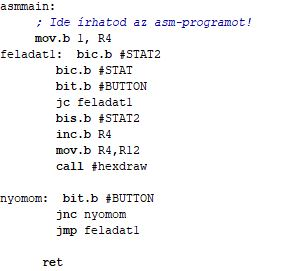
\includegraphics[scale=0.65]{elsodolog}
\centering
\end{figure}

\section{Decimális kiíratás}
A tízes számrendszerbeli számkiíratáshoz az előző programot csak kevéssé kellett módosítanunk. Ehhez a BCD formátumot, és a $dadd$ műveletet használtuk. A parancs úgy végzi el az összeadást, hogy a megjelenő eredmény tízes számrendszerbelinek tűnjön. A papíron történő átváltáshoz hasonlóan a számokat elosztjuk tízzel, majd a maradékokból keletkeznek az átalakított szám számjegyei a hozzájuk tartozó hatványértékekkel. Ha ezeket összeadjuk, megkapjuk a szám decimális értékét. 

\begin{figure}[h]
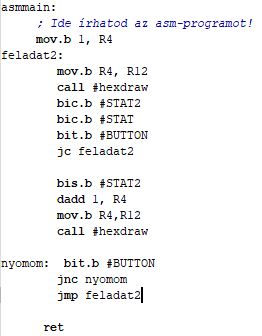
\includegraphics[scale=0.65]{masodikdolog}
\centering
\end{figure}

\section{Joystick irányítás}
A joystick segítségével való irányításhoz az előre definiált irányokat használtuk. A korábbiakhoz hasonlóan vizsgáltuk az egyes irányokba való elmozdítást, ezeknek értékét a carry bitbe tölöttük, majd a jnc parancs segítségével, amennyiben adott irányba való elmozdítás történt, az erre létrehozott mozgatási programrészletekhez ugrottunk. 

\begin{figure}[h]
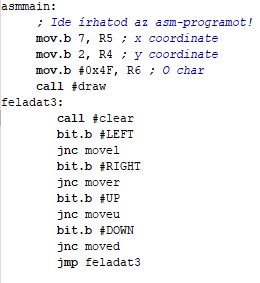
\includegraphics[scale=0.65]{3main}
\centering
\end{figure}


\begin{figure}[h]
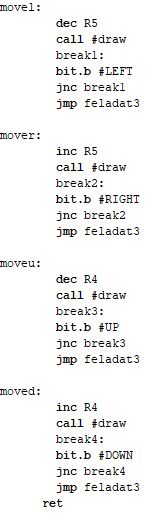
\includegraphics[scale=0.65]{3move}
\centering
\end{figure}

További függvényeket definiáltunk még - draw és clear.  \\
A draw függvény meghívásakor a joystick-al módosítható x és y koordinátákat tartalmazó R4 és R5 regiszterek értékét az R12 és R13 regiszerekbe töltöttük, majd az 'o' karaktert tartalmazó R6 regiszter értékét az R14-be, majd az $LCDChrXY$ valamint az $LCDUpdate$ parancsok hívásával adott pozícióra kiírattuk az LCD-re.
A clear függvény arra szolgált, hogy az előző kirajzolt karaktert felülírja egy szóközzel, így elérve, hogy egy időpontban csak egy kör legyen kirajzolva. 

\begin{figure}[h]
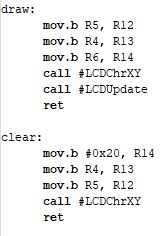
\includegraphics[scale=0.65]{3plus}
\centering
\end{figure}

%Ha szeretnéd hogy az adott fejezet ne legyen számozva használj \section*{} -t, pl Acknowledgements


% Az egyenletekre, táblázatokra, listákra stb. itt nem térnék ki, ahhoz mindenképp érdemes kicsit utána olvasni

% A references mindig a legutolsó fejezet lesz

%  minden hivatkozás elnevezünk, ezzel a névvel fogunk hivatkozni a szövegen belül
% \bibitem{} <- hivatkozásnév
% A hivatkozás formája legjobban a példa dokumentumban látszik a tanárúr honlapján, általában: szerző, olvasott anyag neve, közreműködők, hely, év
% a szövegben pedig \cite{Megadott hivatkozásnév} -vel hivatkozunk


% példa:


% Ez a rész mindig marad:---------
\bibliographystyle{ieeetr}
%\bibliography{references}


% that's all folks
\end{document}
